\documentclass{article}
\usepackage{amsmath}
\usepackage{amsfonts}
\usepackage{amssymb}
\usepackage{multicol}
\usepackage{graphicx}

\graphicspath{ {./images/} }

\setlength{\parindent}{0pt}

\begin{document}

\section*{Review (05/07/2024)}

1. Sketch the graph of $r = -4\cos\theta$.
\\\\
\textbf{Solution:}
\begin{align*}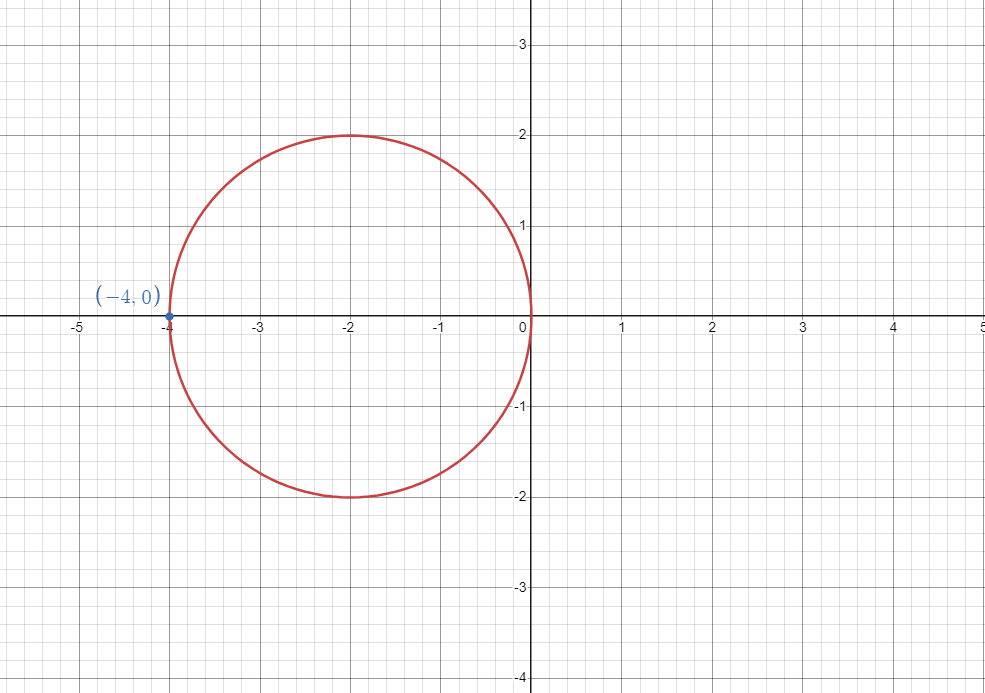
\includegraphics[scale=0.45]{review0507-1.PNG}\end{align*}
\textbf{Alternative way to solve 1:}
\begin{align*}
    r &= -4 \cos \theta \\
    r^2 &= -4 r \cos \theta \\
    &= -4x
\end{align*}
so:
\begin{align*}
    x^2+y^2 = r^2 \rightarrow x^2 + y^2 &= 4x \\
    x^2+4x+y^2 &= 0 \\
    (x^2+4x+4)+y^2 &= 4 && \text{(completing the square)} \\
    (x+2)^2 + y^2 &= 2^2
\end{align*}
essentially, we get an equation of a circle of centre $(-2,0)$ and radius $2$.
\newpage
2. Sketch the graph of $r = 2\cos\theta$ and $r = -2\sin\theta$ on the same coordinate plane.
\\\\
\textbf{Solution:}
\begin{align*}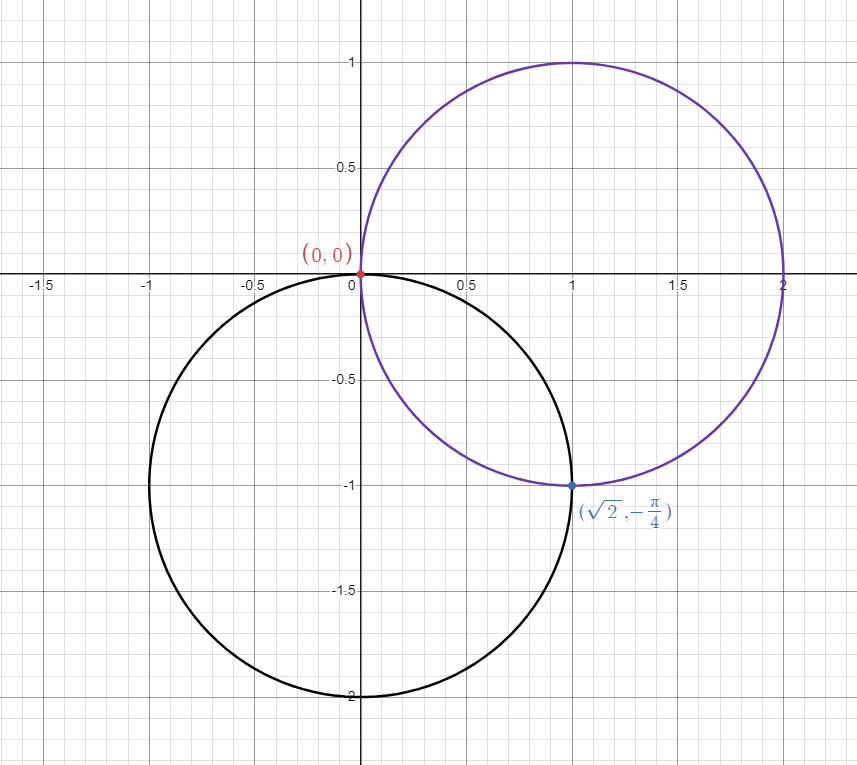
\includegraphics[scale=0.45]{review0507-2.PNG}\end{align*}
To find the intersection points:
\begin{align*}
    2\cos\theta &= -2\sin\theta \\
    -\frac{\sin\theta}{\cos\theta} &= 1 \\
    \tan\theta &= -1 \\
    \theta &= -\frac{\pi}{4}
\end{align*}
and
\begin{align*}
    2\cos(-\frac{\pi}{4}) &= \sqrt{2}
\end{align*}
giving an intersection point of $(\sqrt{2}, -\frac{\pi}{4})$.
\newpage
3. Find the area of the region common to the curves in 2.
\\\\
\textbf{Solution:}
We can take the area of the sin circle from $-\frac{\pi}{4}$ to $0$, and take advantage of the symmetry of the graph.
\begin{align*}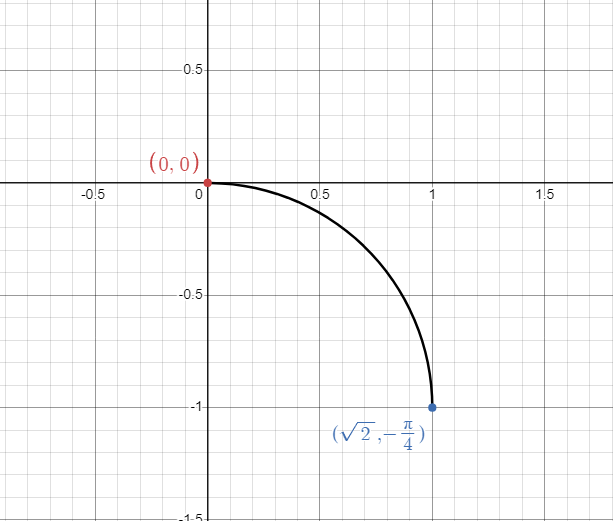
\includegraphics[scale=0.45]{review0507-3.PNG}\end{align*}
\begin{align*}
    A = 2\left(\frac{1}{2} \int_{-\frac{\pi}{4}}^{0}\,(-2\sin\theta)^2\,d\theta\right) &= 4\, \int_{-\frac{\pi}{4}}^{0}\,\sin^2\theta\,d\theta \\
    &= 4\, \int_{-\frac{\pi}{4}}^{0}\, \frac{1-\cos2\theta}{2} \,d\theta \\
    &= 4 \left(\frac{1}{2}\theta - \frac{\sin2\theta}{4} \Bigg|^{0}_{-\frac{\pi}{4}}\right) \\
    &= 4\left(0 - ((\frac{1}{2})(-\frac{\pi}{4})-\frac{\sin2(-\frac{\pi}{4})}{4})\right) \\
    &= \frac{\pi}{2} - 1
\end{align*}

\newpage
4. Sketch a graph of $r = 2\sin3\theta$, then find the area of one petal.
\\\\
\textbf{Solution:}
$n=3$, meaning there are three petals.
\begin{align*}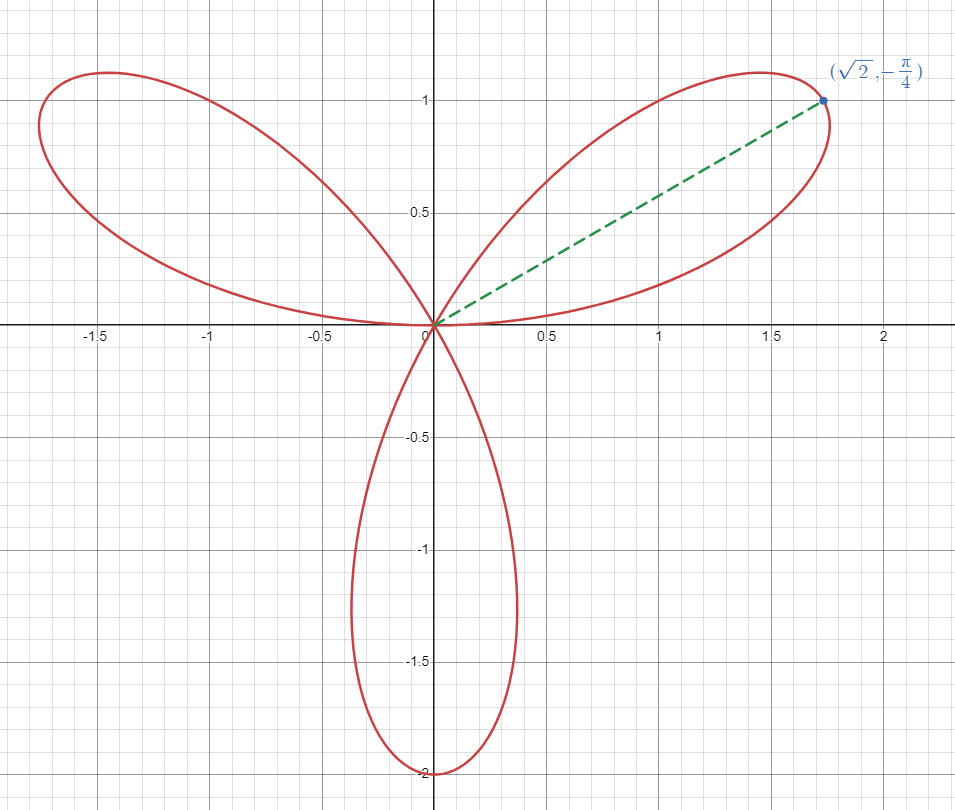
\includegraphics[scale=0.45]{review0507-4.PNG}\end{align*}
Taking advantage of the symmetry:
\begin{align*}
    A = 2\left(\frac{1}{2} \int_{-\frac{\pi}{4}}^{0}\,(-2\sin\theta)^2\,d\theta\right) &= 4\, \int_{-\frac{\pi}{4}}^{0}\,\sin^2\theta\,d\theta \\
    &= 4\, \int_{-\frac{\pi}{4}}^{0}\, \frac{1-\cos2\theta}{2} \,d\theta \\
    &= 4 \left(\frac{1}{2}\theta - \frac{\sin2\theta}{4} \Bigg|^{0}_{-\frac{\pi}{4}}\right) \\
    &= 4\left(0 - ((\frac{1}{2})(-\frac{\pi}{4})-\frac{\sin2(-\frac{\pi}{4})}{4})\right) \\
    &= \frac{\pi}{2} - 1
\end{align*}

\end{document}